\documentclass{article}
\usepackage[utf8]{inputenc}
\usepackage{amsmath}
\usepackage{graphicx}
\usepackage{hyperref}
\usepackage{titling}
\usepackage{enumitem} 

\usepackage{listings}
\usepackage{xcolor} 

\title{\textbf{\Huge LangChain Framework} \\ NLP Course Presentation }
\author{Name: Alireza Dastmalchi Saei}
\date{Stu No.: 993613026}

\pretitle{%
  \begin{center}
  
\includegraphics[width = 150px]{Images/university-of-isfahan-logo.png}\\[\bigskipamount]
  \vspace{3cm}
}
\posttitle{\end{center}}

\lstdefinestyle{pythonstyle}{
    language=Python,
    basicstyle=\ttfamily\small,
    keywordstyle=\color{blue},
    commentstyle=\color{green},
    stringstyle=\color{red},
    showstringspaces=false,
    numbers=left,
    numberstyle=\tiny\color{gray},
    stepnumber=1,
    numbersep=10pt,
    frame=single,
    breaklines=true,
    backgroundcolor=\color{white},
    captionpos=b,
}

\begin{document}
\maketitle

\pagebreak

\tableofcontents

\pagebreak


\section{Introduction}

LangChain is a framework designed for developing applications powered by large language models (LLMs). It streamlines every phase of the LLM application lifecycle, including development, productionization, and deployment.

The aim of this presentation is to introduce class members to the LangChain framework and illustrate how to implement a chatbot using its features. Topics covered in this presentation include various types of memories in chatbots, Chains, Evaluation methods, and Agents.

In the second part, a step-by-step process of implementing a chatbot is provided, which includes Document Loading, Document Splitting, Vectorstores and Embeddings, Retrieval, QnA of custom document, and Chatting with Document.

\vspace{1cm}


\section{LangChain Framework}

LangChain is a framework tailored for applications leveraging large language models (LLMs). Its primary goal is to provide a development environment for LLM applications, addressing key stages from development to deployment.

\subsection{Models, Prompts, and Output Parsers}

LangChain supports both direct API calls to OpenAI and enhanced functionality via its integrated prompts, models, and output parsers. This integration streamlines the development process, allowing for more sophisticated and customizable interactions with LLMs.



\subsubsection{Direct API Calls}
Direct API calls enable straightforward interactions with OpenAI's models. This approach is quick and effective for simple use cases but lacks the flexibility and advanced features provided by LangChain. (For invoking a non-local model, an OpenAI API Token is required!)

\begin{figure}[h]
    \centering
    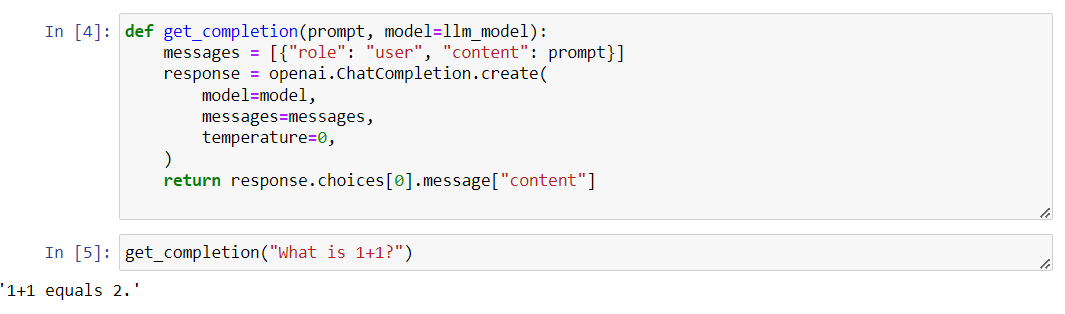
\includegraphics[width=0.8\textwidth]{Images/DirectAPI.png}
    \caption{Direct API Calls}
    \label{fig:example}
\end{figure}



\subsubsection{API Calls through LangChain}
LangChain enhances API calls by incorporating prompts, models, and output parsers:
\begin{itemize}
  \item \textbf{Prompts:} Customizable prompts that guide the LLM in generating desired responses.
  \item \textbf{Models:} Predefined and custom models that can be integrated together.
  \item \textbf{Output Parsers:} Tools to process and structure the raw output from LLMs, making it more usable for specific applications.
\end{itemize}

\begin{figure}[h]
    \centering
    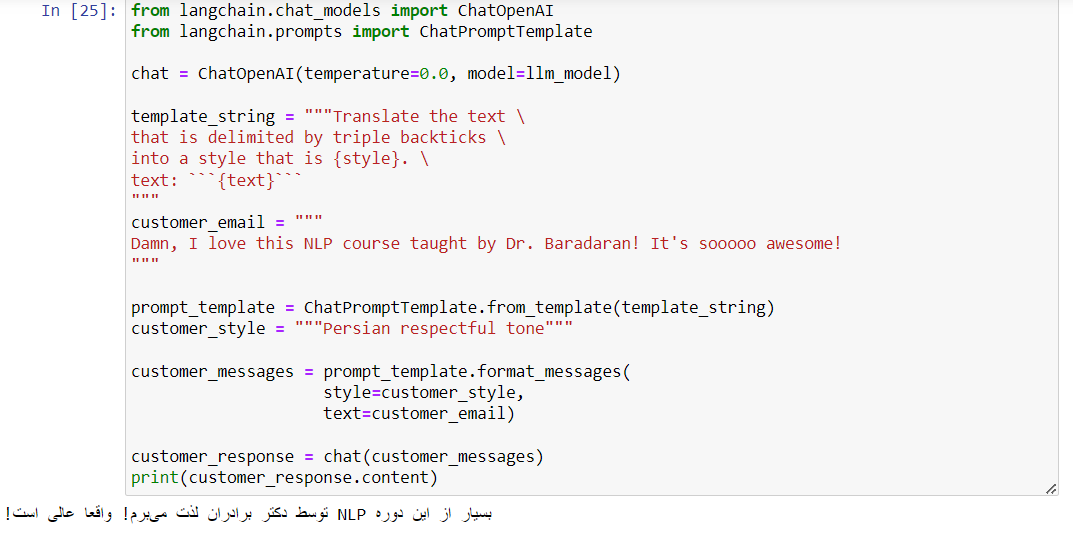
\includegraphics[width=0.8\textwidth]{Images/LangchainAPI.png}
    \caption{Direct API Calls}
    \label{fig:example}
\end{figure}

\bigskip

\begin{figure}[h]
    \centering
    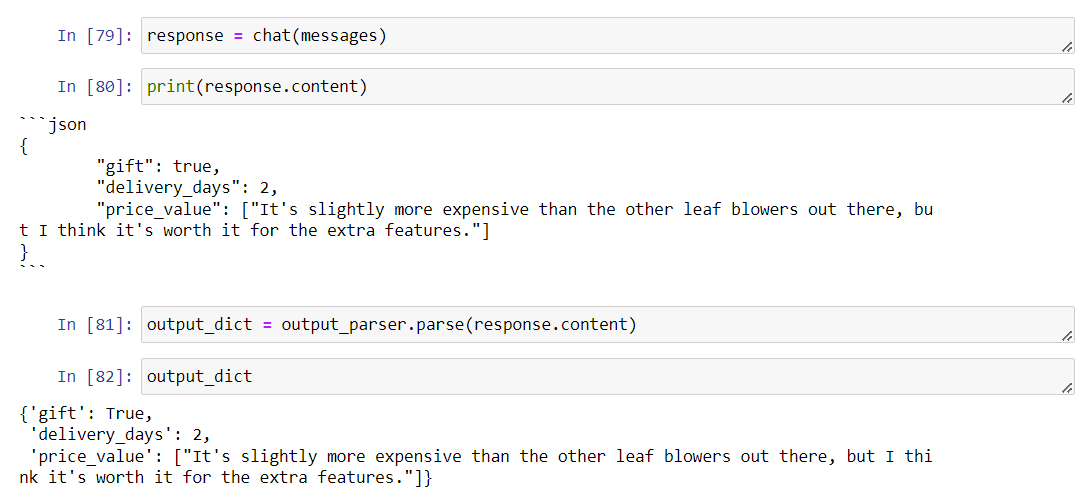
\includegraphics[width=0.8\textwidth]{Images/Parser.png}
    \caption{Parser Usage}
    \label{fig:example}
\end{figure}

\pagebreak

\subsection{Memory}

LLMs are inherently stateless, meaning each transaction is independent of the previous ones. However, for chatbots to simulate memory, the entire conversation context must be provided with each interaction. LangChain offers various memory types to manage and accumulate this conversation context effectively:

\begin{enumerate}[label=\textbf{\arabic*.}, left=0pt, align=left, itemindent=*]
    \setlength{\itemsep}{15pt}
    \item \textbf{ConversationBufferMemory}

    Stores the entire conversation history in a buffer, which is included in every interaction. This method is simple but can become unwieldy with long conversations.

    \item \textbf{ConversationBufferWindowMemory (k)}

    Maintains a sliding window of the last \( k \) interactions. This approach balances memory usage and context relevance by limiting the amount of retained conversation history.

    \item \textbf{ConversationTokenBufferMemory}

    Accumulates conversation context up to a specified token limit. This method ensures the context remains within the LLM's token limit, optimizing memory usage without losing essential information.

    \item \textbf{ConversationSummaryMemory}

    Summarizes the conversation history into a concise format, retaining the most relevant information. This method is efficient for long conversations, as it reduces the amount of context needed while maintaining coherence.
\end{enumerate}

\pagebreak

\subsection{Chains}

Chains in LangChain allow for the sequential processing of inputs through multiple steps, enabling complex workflows and decision-making processes:

\begin{enumerate}[label=\textbf{\arabic*.}, left=0pt, align=left, itemindent=*]
\setlength{\itemsep}{10pt}
    \item \textbf{LLMChain}

    A single chain that processes input through a language model. It is straightforward and useful for simple tasks.

    \item \textbf{Sequential Chains}

    These chains enable multi-step processing, where each step's output serves as the next step's input:
    \begin{itemize}[label=--]
        \item \textbf{SimpleSequentialChain:} A basic sequential chain with a fixed order of steps.
        \item \textbf{SequentialChain:} A more flexible chain allowing for conditional branching and complex workflows.
    \end{itemize}

    \item \textbf{Router Chain}

    Directs inputs to different chains based on specific criteria. This chain type is useful for applications requiring dynamic decision-making.
\end{enumerate}

\bigskip

\subsection{Q\&A over Documents}

LangChain processes inputs through embedding techniques, transforming raw text into vector representations for efficient similarity searches across document repositories. By reading and interpreting data directly from documents, LangChain enhances the bot's ability to provide accurate and contextually relevant responses.

\begin{figure}[h]
    \centering
    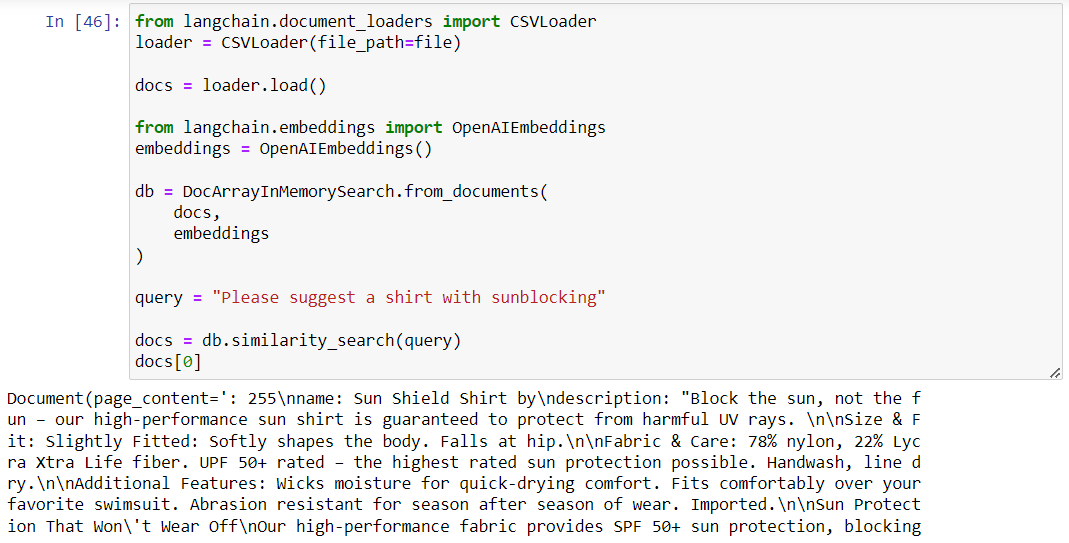
\includegraphics[width=0.75\textwidth]{Images/QA.png}
    \caption{Simple QA System}
    \label{fig:example}
\end{figure}

\pagebreak

\subsection{Evaluation}

LangChain provides several methods to evaluate and improve models, ensuring robust and accurate performance:

\begin{enumerate}[label=\textbf{\arabic*.}, left=0pt, align=left, itemindent=*]
    \item \textbf{Example Generation}

    Generates examples to test and refine models. These examples can be hard-coded or generated by the LLM.

    \item \textbf{Manual Evaluation and Debugging}

    Involves human evaluators assessing the model's performance and identifying areas for improvement.

    \item \textbf{LLM-assisted Evaluation}

    Utilizes LLMs to assist in the evaluation process, automating parts of the assessment and providing insights.

    \item \textbf{LangChain Evaluation Platform}

    A dedicated platform for evaluating models, offering tools and metrics to measure performance comprehensively.
\end{enumerate}

\vspace{3cm}

\subsection{Agents}

Agents in LangChain can utilize built-in tools or custom-defined tools to enhance functionality:

\subsubsection{Built-in Tools}
LangChain offers several pre-built tools for common tasks:
\begin{itemize}
  \item \textbf{DuckDuckGo Search:} Enables web search capabilities.
  \item \textbf{Wikipedia:} Accesses information from Wikipedia.
  \item \textbf{Python (PythonREPLTool):} Executes Python code.
\end{itemize}

\subsubsection{Custom Tools}
Users can define their own tools to meet specific requirements, extending the framework's versatility.

\section{Retrieval-Augmented Generation (RAG)}

Retrieval-Augmented Generation (RAG) combines traditional information retrieval systems with generative LLMs, enhancing their ability to provide contextually relevant responses.

\bigskip
\bigskip

\subsection{Overview}

RAG frameworks leverage external datasets to retrieve contextual documents as part of the LLM's execution process. This approach is beneficial for applications requiring specific document references, such as technical support and content summarization.

\bigskip
\bigskip

\subsection{Document Loading}

Documents can be loaded from various sources, ensuring flexibility and broad applicability:

\begin{enumerate}[label=\textbf{\arabic*.}, left=0pt, align=left, itemindent=*]
    \item \textbf{PDF}

    Each page in a PDF is treated as a separate document, capturing its content and metadata.

    \item \textbf{URLs}

    Documents can be retrieved from web URLs, enabling dynamic and up-to-date information access.

    \item \textbf{YouTube}

    Video content can be transcribed and treated as documents, allowing for multimedia interaction.

    \item \textbf{Notion}

    Integrates with Notion to retrieve documents, leveraging its robust content management capabilities.
    
    \item \textbf{XML}
    
    \item \textbf{JSON}
\end{enumerate}

\bigskip
\bigskip

\subsection{Document Splitting}

Documents are split into smaller chunks while retaining meaningful relationships. This step is crucial for efficient processing and accurate retrieval. Various text splitters are available in LangChain to handle different types of documents:

\begin{enumerate}[label=\textbf{\arabic*.}, left=0pt, align=left, itemindent=*]
    \item \textbf{CharacterTextSplitter}

    Splits text based on character count.

    \item \textbf{MarkdownHeaderTextSplitter}

    Splits text based on markdown headers.

    \item \textbf{Context Aware Splitter}

    Maintains context by splitting at logical boundaries.

    \item \textbf{TokenTextSplitter}

    Splits text into tokens, useful for LLMs with token-based context windows.

    \item \textbf{SentencesTransformersTokenTextSplitter}

    Splits text using sentence transformers, enhancing context retention.

    \item \textbf{RecursiveCharacterTextSplitter}

    Recursively splits text to maintain context.

    \item \textbf{NLTKTextSplitter}

    Utilizes the Natural Language Toolkit (NLTK) for splitting.

    \item \textbf{SpacyTextSplitter}

    Uses the Spacy library for text splitting.
\end{enumerate}

\pagebreak

\subsection{Storage}

Embeddings capture the context and meaning of text, enabling efficient and relevant information retrieval:

\begin{enumerate}[label=\textbf{\arabic*.}, left=0pt, align=left, itemindent=*]
    \item \textbf{Embeddings}

    Embedding vectors represent the semantic meaning of text. Similar contexts will have similar vectors, facilitating accurate retrieval.

    \item \textbf{Vector Store}

    A storage system where all document splits are converted into embedding vectors. The vector store can find and return the top \textit{n} similar embeddings to an input query. Duplicate data may cause the vector store to return duplicate answers, highlighting the need for careful data management.
\end{enumerate}

\bigskip
\bigskip

\subsection{Retrieval}

Retrieval is the core of the RAG flow, enabling the system to find relevant information based on input queries:

\begin{enumerate}[label=\textbf{\arabic*.}, left=0pt, align=left, itemindent=*]
    \item \textbf{Addressing Diversity}

    Maximum Marginal Relevance (MMR) fetches diverse results, enhancing the breadth of retrieved information.

    \item \textbf{Addressing Specificity}

    Metadata filters and self-query retrievers refine results based on specific criteria, ensuring relevance and accuracy.

    \item \textbf{Additional Tricks}

    Contextual compression retrievers compress results to fit within context limits, maintaining information integrity.
\end{enumerate}

\bigskip

\subsection{Chat with Data}

LangChain supports interactive querying and chatting with documents through the RetrievalQA chain. This process involves using PromptTemplates and methods to resolve short context issues, such as Map Reduce, Refine, and Map Re-rank, to ensure comprehensive and coherent responses.

\pagebreak

\section{Implementation}

In this part, we will go through the code for implementing a chatbot to chat with custom uploaded document. The overview of the process can be seen below:

\begin{figure}[h]
    \centering
    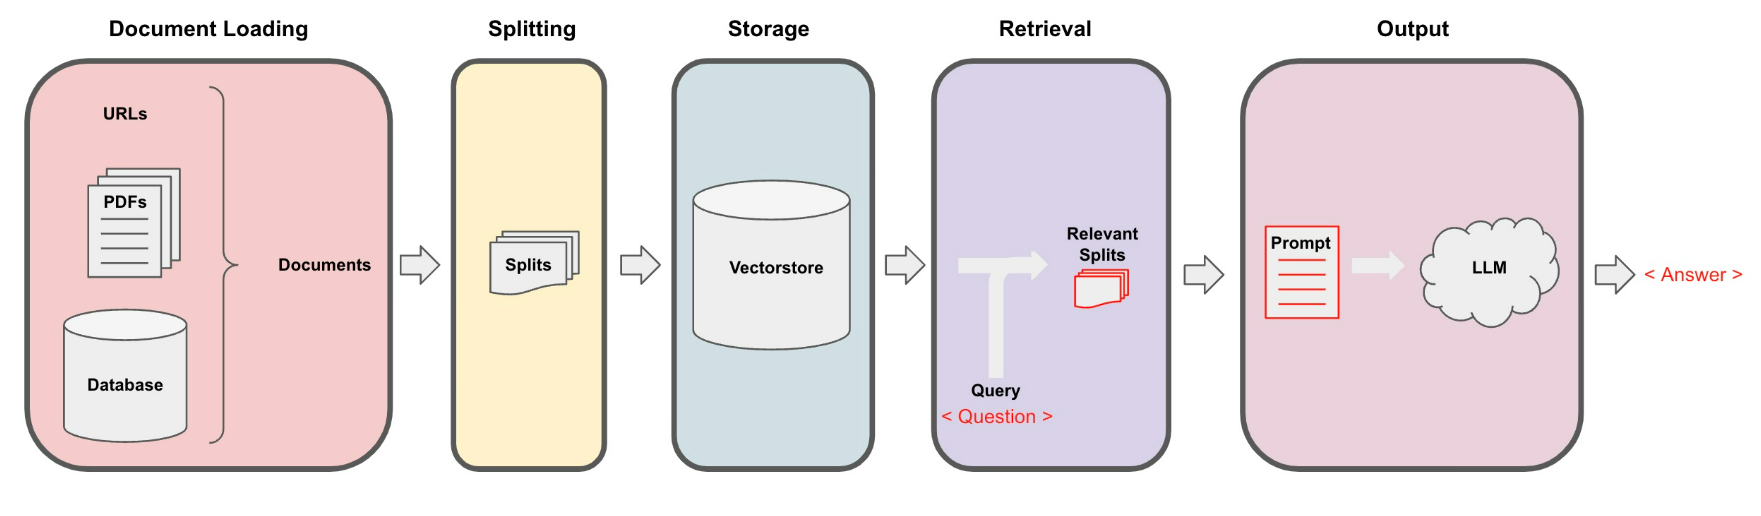
\includegraphics[width=1\textwidth]{Images/Process.png}
    \caption{Implementation Process}
    \label{fig:example}
\end{figure}


\vspace{4cm}


\subsection{Import required libraries}:

\begin{lstlisting}[style=pythonstyle, caption={Python Code for OpenAI API Key Setup}]
import os
import openai
import sys
sys.path.append('../..')

import panel as pn  # GUI
pn.extension()

from dotenv import load_dotenv, find_dotenv
_ = load_dotenv(find_dotenv()) # read local .env file

openai.api_key = os.environ['OPENAI_API_KEY']
\end{lstlisting}

\pagebreak

\subsection{Custom Model as Conversational Agent}

\begin{lstlisting}[style=pythonstyle, caption={Custom Chat Model with LangChain}]
from langchain.vectorstores import Chroma
from langchain.embeddings.openai import OpenAIEmbeddings

persist_directory = 'docs/chroma/'
embedding = OpenAIEmbeddings()
vectordb = Chroma(persist_directory=persist_directory, embedding_function=embedding)

question = "What are major topics for this class?"
docs = vectordb.similarity_search(question, k=3)
len(docs)

from langchain.chat_models import ChatOpenAI
llm = ChatOpenAI(model_name=llm_name, temperature=0)
llm.predict("Hello world!")


from langchain.prompts import PromptTemplate
template = """Use the following pieces of context to answer the question at the end.
If you don't know the answer, just say that you don't know, don't try to make up an answer.
Use three sentences maximum. Keep the answer as concise as possible.
Always say "thanks for asking!" at the end of the answer.
{context}
Question: {question}
Helpful Answer:"""
QA_CHAIN_PROMPT = PromptTemplate(input_variables=["context", "question"], template=template)

from langchain.chains import RetrievalQA
question = "Is probability a class topic?"
qa_chain = RetrievalQA.from_chain_type(llm,
                                       retriever=vectordb.as_retriever(),
                                       return_source_documents=True,
                                       chain_type_kwargs={"prompt": QA_CHAIN_PROMPT})

result = qa_chain({"query": question})
result["result"]
\end{lstlisting}

\pagebreak

\subsection{Memory}

\begin{lstlisting}[style=pythonstyle, caption={Import and Define Memory}]

from langchain.memory import ConversationBufferMemory
memory = ConversationBufferMemory(
    memory_key="chat_history",
    return_messages=True
)

\end{lstlisting}

\bigskip

\subsection{ConversationalRetrievalChain}

\begin{lstlisting}[style=pythonstyle, caption={Conversational Retrieval Chain Setup}]
from langchain.chains import ConversationalRetrievalChain

# Set up the retriever from the vector store
retriever = vectordb.as_retriever()

# Initialize the conversational retrieval chain with memory
qa = ConversationalRetrievalChain.from_llm(
    llm,
    retriever=retriever,
    memory=memory
)

# Ask a question and get the result
question = "Is probability a class topic?"
result = qa({"question": question})
print(result['answer'])

# Ask another question related to the previous context
question = "Why are those prerequisites needed?"
result = qa({"question": question})
print(result['answer'])
\end{lstlisting}

\pagebreak

\subsection{Create a chatbot that works on your documents}

\begin{lstlisting}[style=pythonstyle, caption={Import required libraries}]

from langchain.embeddings.openai import OpenAIEmbeddings
from langchain.text_splitter import CharacterTextSplitter, RecursiveCharacterTextSplitter
from langchain.vectorstores import DocArrayInMemorySearch
from langchain.document_loaders import TextLoader
from langchain.chains import RetrievalQA,  ConversationalRetrievalChain
from langchain.memory import ConversationBufferMemory
from langchain.chat_models import ChatOpenAI
from langchain.document_loaders import TextLoader
from langchain.document_loaders import PyPDFLoader

\end{lstlisting}


\subsection{Loading Database and Conversational Retrieval Chain}

\begin{lstlisting}[style=pythonstyle, caption={Python Code for Loading Database and Creating a Conversational Retrieval Chain}]
def load_db(file, chain_type, k):
    # load documents
    loader = PyPDFLoader(file)
    documents = loader.load()
    # split documents
    text_splitter = RecursiveCharacterTextSplitter(chunk_size=1000, chunk_overlap=150)
    docs = text_splitter.split_documents(documents)
    # define embedding
    embeddings = OpenAIEmbeddings()
    # create vector database from data
    db = DocArrayInMemorySearch.from_documents(docs, embeddings)
    # define retriever
    retriever = db.as_retriever(search_type="similarity", search_kwargs={"k": k})
    # create a chatbot chain. Memory is managed externally.
    qa = ConversationalRetrievalChain.from_llm(
        llm=ChatOpenAI(model_name=llm_name, temperature=0),
        chain_type=chain_type,
        retriever=retriever,
        return_source_documents=True,
        return_generated_question=True,
    )
    return qa
\end{lstlisting}

\pagebreak

\subsection{Class and Dashboard Implementation}

\begin{lstlisting}[style=pythonstyle, caption={Python Code for Class and Dashboard Implementation}]
import panel as pn
import param

class cbfs(param.Parameterized):
    chat_history = param.List([])
    answer = param.String("")
    db_query  = param.String("")
    db_response = param.List([])

    def __init__(self,  **params):
        super(cbfs, self).__init__( **params)
        self.panels = []
        self.loaded_file = "docs/cs229_lectures/MachineLearning-Lecture01.pdf"
        self.qa = load_db(self.loaded_file,"stuff", 4)

    def call_load_db(self, count):
        if count == 0 or file_input.value is None:  # init or no file specified :
            return pn.pane.Markdown(f"Loaded File: {self.loaded_file}")
        else:
            file_input.save("temp.pdf")  # local copy
            self.loaded_file = file_input.filename
            button_load.button_style="outline"
            self.qa = load_db("temp.pdf", "stuff", 4)
            button_load.button_style="solid"
        self.clr_history()
        return pn.pane.Markdown(f"Loaded File: {self.loaded_file}")

    def convchain(self, query):
        if not query:
            return pn.WidgetBox(pn.Row('User:', pn.pane.Markdown("", width=600)), scroll=True)
        result = self.qa({"question": query, "chat_history": self.chat_history})
        self.chat_history.extend([(query, result["answer"])])
        self.db_query = result["generated_question"]
        self.db_response = result["source_documents"]
        self.answer = result['answer']
        self.panels.extend([
            pn.Row('User:', pn.pane.Markdown(query, width=600)),
            pn.Row('ChatBot:', pn.pane.Markdown(self.answer, width=600, style={'background-color': '#F6F6F6'}))
        ])
        inp.value = ''  #clears loading indicator when cleared
        return pn.WidgetBox(*self.panels,scroll=True)

    @param.depends('db_query ', )
    def get_lquest(self):
        if not self.db_query :
            return pn.Column(
                pn.Row(pn.pane.Markdown(f"Last question to DB:", styles={'background-color': '#F6F6F6'})),
                pn.Row(pn.pane.Str("no DB accesses so far"))
            )
        return pn.Column(
            pn.Row(pn.pane.Markdown(f"DB query:", styles={'background-color': '#F6F6F6'})),
            pn.pane.Str(self.db_query )
        )

    @param.depends('db_response', )
    def get_sources(self):
        if not self.db_response:
            return
        rlist=[pn.Row(pn.pane.Markdown(f"Result of DB lookup:", styles={'background-color': '#F6F6F6'}))]
        for doc in self.db_response:
            rlist.append(pn.Row(pn.pane.Str(doc)))
        return pn.WidgetBox(*rlist, width=600, scroll=True)

    @param.depends('convchain', 'clr_history')
    def get_chats(self):
        if not self.chat_history:
            return pn.WidgetBox(pn.Row(pn.pane.Str("No History Yet")), width=600, scroll=True)
        rlist=[pn.Row(pn.pane.Markdown(f"Current Chat History variable", styles={'background-color': '#F6F6F6'}))]
        for exchange in self.chat_history:
            rlist.append(pn.Row(pn.pane.Str(exchange)))
        return pn.WidgetBox(*rlist, width=600, scroll=True)

    def clr_history(self,count=0):
        self.chat_history = []
        return
\end{lstlisting}

\pagebreak

\subsection{Dashboard}

\begin{lstlisting}[style=pythonstyle, caption={Python Code for Dashboard Implementation}]
cb = cbfs()

file_input = pn.widgets.FileInput(accept='.pdf')
button_load = pn.widgets.Button(name="Load DB", button_type='primary')
button_clearhistory = pn.widgets.Button(name="Clear History", button_type='warning')
button_clearhistory.on_click(cb.clr_history)
inp = pn.widgets.TextInput( placeholder='Enter text here')

bound_button_load = pn.bind(cb.call_load_db, button_load.param.clicks)
conversation = pn.bind(cb.convchain, inp)

jpg_pane = pn.pane.Image( './img/convchain.jpg')

tab1 = pn.Column(
    pn.Row(inp),
    pn.layout.Divider(),
    pn.panel(conversation,  loading_indicator=True, height=300),
    pn.layout.Divider(),
)
tab2= pn.Column(
    pn.panel(cb.get_lquest),
    pn.layout.Divider(),
    pn.panel(cb.get_sources ),
)
tab3= pn.Column(
    pn.panel(cb.get_chats),
    pn.layout.Divider(),
)
tab4=pn.Column(
    pn.Row( file_input, button_load, bound_button_load),
    pn.Row( button_clearhistory, pn.pane.Markdown("Clears chat history. Can use to start a new topic" )),
    pn.layout.Divider(),
    pn.Row(jpg_pane.clone(width=400))
)
dashboard = pn.Column(
    pn.Row(pn.pane.Markdown('# ChatWithYourData_Bot')),
    pn.Tabs(('Conversation', tab1), ('Database', tab2), ('Chat History', tab3),('Configure', tab4))
)
dashboard
\end{lstlisting}

\pagebreak

\section{Explanation Video Link}

You can access the explanation video (in Farsi) using the following \href{https://drive.google.com/drive/folders/1g1kx0Zp5GgZeXSWjRwog4qBefWNBcyHA?usp=drive_link}{link}.


\end{document}
